\chapter{Modelo de representación datos para SR}
\label{capitulo:modelo}

% % introducción del capítulo
En este capítulo se presenta un modelo para la representación de datos en SR. Se comienza con una revisión exhaustiva sobre la evolución de representaciones de datos para SR mostrando sus ventajas y desventajas. Posteriormente a partir de las deficiencias encontradas se propone un nuevo modelo. Finalmente, se realiza una discusión respecto al modelo propuesto en comparación a otros.

\section{Trabajo relacionado}
\label{modelo:trabajorelacionado}

% % Introducción de la sección trabajo  relacionado
Los SR están en constante evolución y los atributos que participan en las interacciones entre los usuarios e ítems son cada vez más variadas (Palomino 2012). Las relaciones existentes entre la inteligencia colectiva y los SR no está clara. Cabe destacar que los SR son capaces de “capturar” la inteligencia colectiva para generar recomendaciones que son de utilidad para los usuarios. El área de los sistema colaborativos reconoce que las distintas actividades no son eventos aislados sino que se sitúan dentro de un contexto que informa su sentido y carácter \citep{Suchman:1987}.

Los eventos representan la base de los SR que permite obtener relaciones entre usuarios e ítems y así realizar el cálculo de una recomendación para el usuario activo. Estos se basan principalmente en las interacciones de los usuarios hacia los ítems que son reflejadas en los sistemas mediante eventos.

Sea $C$ el conjunto de usuarios, $S$ el conjunto de ítems, un evento se define como la siguiente tupla:
\begin{equation}
\label{def:evento}
	e = \{ (u,i,v) | s \in C, i \in S, v\, alg\acute{u}n\, valor  \}
\end{equation}



El valor $v$ corresponde a una preferencia del usuario y puede ser de distintos tipos dependiendo de las posibles interacciones del dominio de aplicación. Puede corresponder a una valoración numérica,  comentario, etiqueta, \textit{like}, etc. Por ejemplo, el valor de un evento \textit{Rating} en \textit{Movielens} se define en el dominio real entre 1 y 5. En otros casos como \textit{Delicious}\footnote{https://delicious.com/} el valor del evento pertenece al conjunto de combinaciones alfanuméricas que representa el \textit{tag} que un usuario asigna a un \textit{bookmark}. Se asume que una preferencia de un usuario a un ítem es única, luego se define $E$ como el conjunto de todos los eventos de un sistema.

%Párrafo que hable sobre Lenskit y su representación, definición de historias de Usuario.
\cite{Ekstrand:2011} en su herramienta para construir, investigar y estudiar SR de filtrado colaborativo \textit{Lenskit}\footnote{http://lenskit.grouplens.org/} utilizan una representación básica de eventos de  \textit{rating}. En su trabajo definen el concepto de historia de usuario que corresponde a un subconjunto de eventos ordenados temporalmente relacionados a un usuario específico. Formalmente $H=(\mathcal{P}(E), \prec)$ donde $H$ es una historia para el usuario $u$, $E$ el conjunto de todos los eventos y $\prec$ una relación de orden temporal entre los eventos.

La representación básica de evento que considera solo al usuario e ítem no permite:
%Dificultades
\begin{itemize}
	\item Describir un conjunto de interacciones sobre el mismo ítem \citep{Babar:2010}, por ejemplo no se puede representar un \textit{rating} y \textit{tag} sobre un mismo ítem. Disponer de una representación de este tipo permite a los SR aprovechar los diversos comportamientos que tienen los usuarios hacia un mismo ítem.
	\item El evento posee escasa información referente al contexto donde fue efectuado. Un tipo de información que es representada es una marca temporal del evento que permite situarlo en el tiempo, entregando información al SR sobre el contexto \citep{Adomavicius:2011}.
	%\item Un evento no está situado dentro de un contexto temporal, social o espacial. Estos tres tipos de contexto (implícitamente sin ningún \textit{framework} subyacente) han permitido a los SR mejorar la calidad de las recomendaciones.
	\item Modelar la información social referente a la Web 2.0 que proporciona nuevas formas de interacción hacia los ítems \citep{Bobadilla:2013}.
\end{itemize}


%Definición con agregación de múltiples dimensiones datawarehousing.

Dado lo anterior aparecen trabajos que tratan de abordar estas dificultades. \cite{Adomavicius:2001} presentan un modelo multidimensional basado en \textit{data warehousing} que permite representar dimensiones adicionales a las clásicas usuario e ítem. El modelo supone que una interacción entre usuario e ítem depende de múltiples dimensiones. En este trabajo se basan en eventos de valoración numérica, luego definen la función $R$:

\begin{equation}
\label{modelo:olap}
	R: D_1 \times D_2 \times D_3 \times D_4 \times \cdots \times D_n \rightarrow ratings
\end{equation}

% % revisar la validez de este parrafo
Este modelo resuelve el problema de utilizar data multi-dimensional en SR y permite situar las interacciones de un usuario en distintos contextos. Sin embargo, su implementación es compleja debido a la utilización de agregaciones jerárquicas (\textbf{OLAP}) y un lenguaje de consultas llamado \textbf{RQL} \citep{Palomino:2012}.

%Definición de CARS.
Varios trabajos señalan la importancia de utilizar información contextual en el proceso de recomendación \citep{Adomavicius:2005:2}, \citep{Adomavicius:2001}, \citep{Adomavicius:2011}, \citep{Palomino:2012} y \citep{Zhang:2010}. Dado lo anterior, \cite{Adomavicius:2011} definen  los \textbf{CARS} \textit{(Context Aware Recommender Systems)} (véase sección \ref{marco:cars}) como SR que utilizan información contextual para la predicción de valoraciones numéricas. Formalmente se define la función de $R$:

\begin{equation}
\label{modelo:cars}
	R: User \times Item \times Contexto  \rightarrow ratings
\end{equation}

%Definición sobre eventos del tipo tags.
Tanto la representación que realizan \cite{Adomavicius:2001} en la definición \eqref{modelo:olap} y  \cite{Adomavicius:2011} en la definición \eqref{modelo:cars} son válidas solo para SR basados en eventos de valoración numérica(\textit{ratings}). Sin embargo, la aparición de la Web 2.0 ha otorgado nuevas formas de interacción para los usuarios como etiquetas (\textit{tagging}), \textit{liking}, \textit{commenting}, \textit{following}, etc. En particular, la información referente a los \textit{tags} se ha modelado mediante la extensión de la matriz item-usuario a un cubo ítems-usuarios-tags \citep{Song:2011}.

%Definición propuesta por Synergy.
Con el objetivo de modelar las nuevas interacciones, \cite{Babar:2010} presentan \textit{Synergy} una herramienta para la creación, ejecución y comparación de diferentes algoritmos de filtrado colaborativo. \textit{Synergy} esta construido en base a dos tipos de eventos \textit{rating} y \textit{tagging}, permitiendo la hibridación de algoritmos utilizando estos dos tipos de eventos. Para modelar diversas formas de interacción y abstraerse del dominio de aplicación proponen el modelo conceptual de la Figura \ref{fig:modeloconceptualsynergy}. 

\begin{figure}[tp]
	\centering
	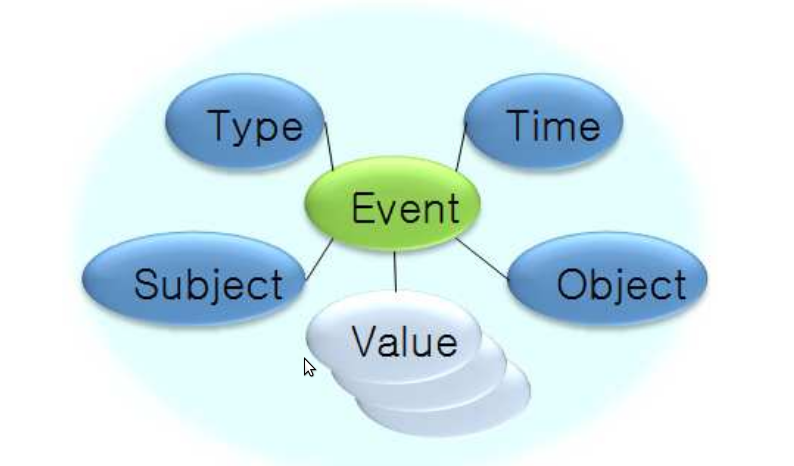
\includegraphics[scale=.3]{images/modelosinergy.png}
	\caption{Modelo conceptual de \textit{Synergy} tomado de \citep{Babar:2010}}
	\label{fig:modeloconceptualsynergy}
\end{figure}

El modelo de \textit{Synergy} se define de la siguiente forma:

\begin{equation}
\label{modelo:eqsynergy}
\begin{split}
\begin{aligned}
	&U = \{u_1, u_2,\cdots,u_n\}\\
	&C = \{c_1, c_2,\cdots,c_n\}\\
	&I = \{i_1, i_2,\cdots,i_n\}\\
	&E = \{(s, p, o, t) | s\in U, p \in I, o \in C, &t\, es\, el\, tiempo\}\\
	&V = \{(e, a) | e \in E, a\, es\, alg\acute{u}n\, valor\}\\
\end{aligned}
\end{split}
\end{equation}

Donde $U$ es el conjunto de todos los usuarios, $C$ de todos los ítems, $I$ de todas las posibles interacciones, $E$ de eventos y $V$ los valores que puede tomar un evento. Este modelo conceptual es plasmado en el diagrama entidad-relación de la Figura \ref{fig:dersynergy} que permite almacenar los datos dentro de una base de datos relacional. La principal ventaja de este modelo es su flexibilidad para describir varios tipos de interacciones, sin embargo no permite situarlas dentro de un contexto espacial y social.

\begin{figure}[tp]
	\centering
	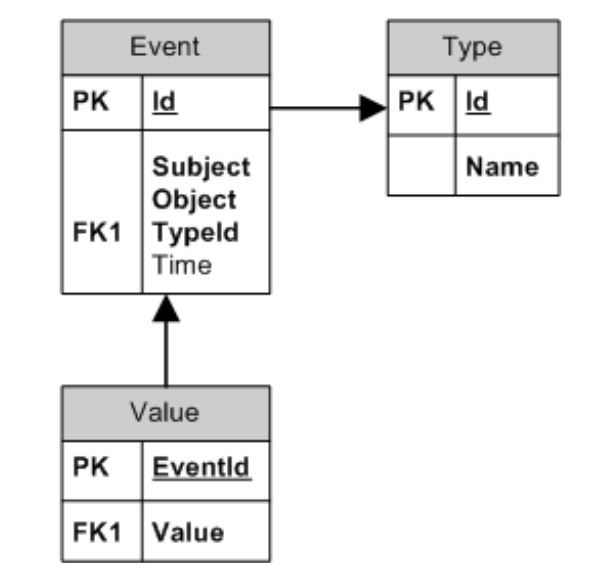
\includegraphics[scale=.3]{images/dersynergy.png}
	\caption{Diagrama entidad-relación \textit{Synergy} tomado de \citep{Babar:2010}}
	\label{fig:dersynergy}
\end{figure}

%Definición propuesta por Palomino.

\cite{Palomino:2012} presenta un modelo conceptual que extiende de \textit{Synergy} basándose en el \textit{framework} conceptual \textit{3-Ontology}. En este modelo sitúa los eventos dentro de un lugar y una comunidad. En la definición \ref{modelo:eqpalomino} se define formalmente la representación, donde $S$ son las comunidades. En la Figura \ref{fig:modeloconceptualpalomino} se muestra el modelo conceptual propuesto por \cite{Palomino:2012}. Al igual que en \textit{Synergy} se desarrolla un diagrama entidad-relación para almacenar la información (véase Figura \ref{fig:derpalomino}).

\begin{equation}
\label{modelo:eqpalomino}
\begin{split}
\begin{aligned}
	&U = \{u_1, u_2,\cdots,u_n\}\\
	&C = \{c_1, c_2,\cdots,c_n\}\\
	&I = \{i_1, i_2,\cdots,i_n\}\\
	&S = \{s_1, s_2,\cdots,s_n|S\subseteq U\}\\
	&E = \{(s, p, o, t, y, l) | s\in U, p \in I, o \in C, t\, es\, el\, tiempo, y \in S, l\, es\, el\, lugar\}\\
	&V = \{(e, a) | e \in E, a\, es\, alg\acute{u}n\, valor\}
\end{aligned}
\end{split}
\end{equation}

\begin{figure}[tp]
	\centering
	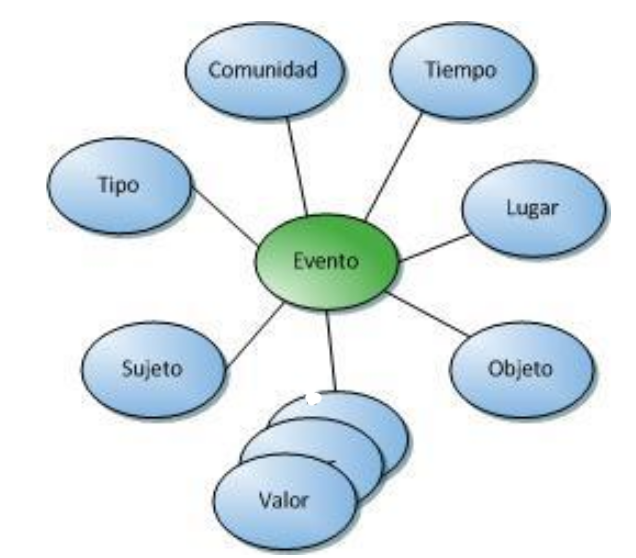
\includegraphics[scale=.3]{images/modelo-palomino.png}
	\caption{Modelo conceptual de \textit{Synergy} tomado de \citep{Palomino:2012}}
	\label{fig:modeloconceptualpalomino}
\end{figure}

\begin{figure}[tp]
	\centering
	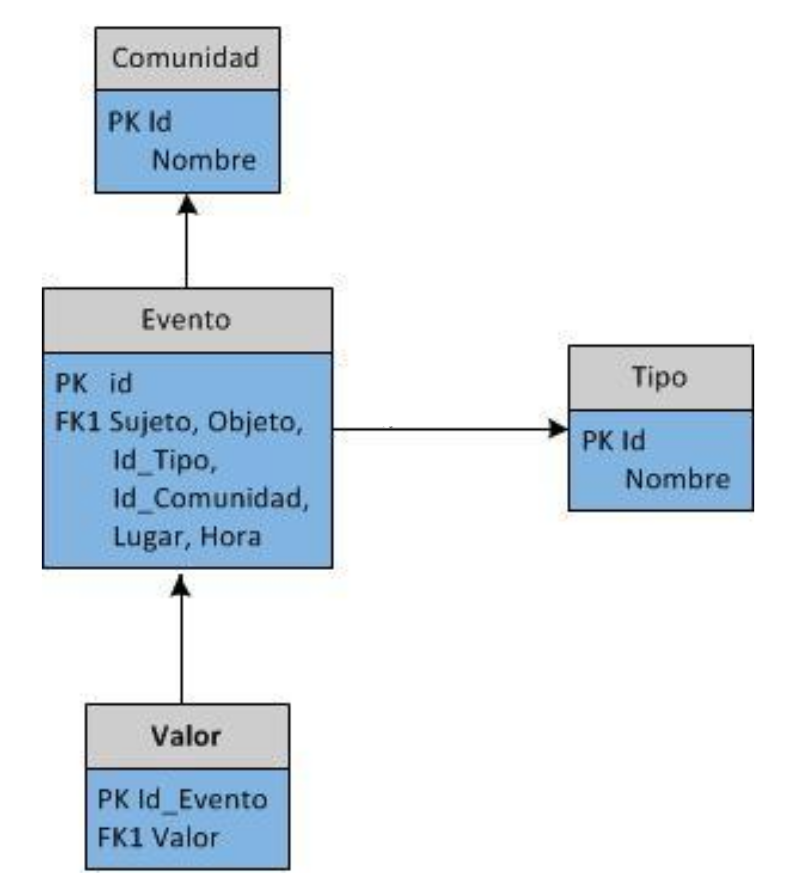
\includegraphics[scale=.3]{images/derpalomino.png}
	\caption{Diagrama entidad-relación tomado de \cite{Palomino:2012}}
	\label{fig:derpalomino}
\end{figure}

El trabajo de Palomino permite describir las interacciones que suceden dentro de una red social basado en el \textit{framework} conceptual \textit{3-ontology}. Sin embargo, el modelo presenta las siguientes deficiencias: 

\begin{itemize}
	\item Es solo un modelo conceptual que no posee una implementación concreta.
	\item No permite modelar los perfiles del usuario, ítem, comunidad y lugar.
	\item No modela las tres formas representaciones de la \textit{3-Ontology} trazas, retratos y mapas.
	\item No modela explícitamente las relaciones existentes entre los tres contenedores de sentido de la \textit{3-ontology}.
\end{itemize}

\section{Modelo de representación de interacciones para SR basado en la 3-Ontology}

En esta sección se presenta un modelo de representación de interacciones para SR basado en la \textit{3-Ontology} que tiene como objetivo modelar las características de los SR modernos.

\subsection{Contenedores de sentido de la 3-Ontology}

Los SR utilizan la información de ambientes colaborativos donde los usuarios interactúan entre sí y con ítems. Dado esto el \textit{framework 3-Ontology} define tres contenedores de sentido eventos, comunidades y lugares (véase sección \ref{marco:3ontology}) para situar las interacciones dentro de un contexto social, temporal y espacial. El modelo conceptual propuesto se presenta en el diagrama entidad-relación de la Figura \ref{fig:derpropuesto}. Se pueden observar las relaciones existentes entre los elementos básicos de los SR y los contenedores de sentido de la \textit{3-Ontology}.

\begin{figure}[tp]
	\centering
	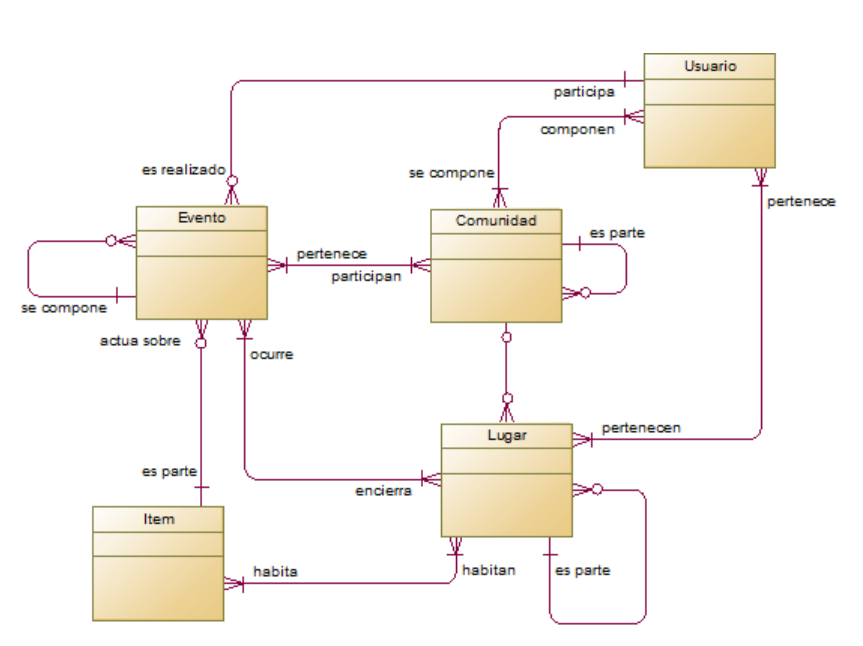
\includegraphics[scale=.4]{images/derpropuesto.png}
	\caption{Modelo conceptual propuesto}
	\label{fig:derpropuesto}
\end{figure}

A continuación se definen formalmente cada uno de los elementos básicos usuario e ítem y los contenedores de sentido de la \textit{3-Ontology}.

\subsubsection{Usuarios e \'items}

Los usuarios son quienes asignan su preferencia a un ítem. Esta puede ser de distintos tipos dependiendo del dominio de aplicación. Cada usuario tiene un conjunto de atributos como nombre, fecha de nacimiento, información demográfica, en general. Los primeros SR se basaban en este conjunto de atributos para realizar recomendaciones.

Se define formalmente un usuario $u$, donde $attr_i^{u}$ es un atributo del usuario que posee un conjunto de valores dependiendo del dominio de aplicación:

\begin{equation}
\label{modelo:user}
	u = (attr_1^{u},\,attr_2^{u},\,attr_3^{u},\cdots,\,attr_n^{u})
\end{equation}

Los ítems son objetos a los cuales el usuario asigna una preferencia. Son de distinto tipo y dependen del dominio de aplicación, por ejemplo en \textit{Movielens} son películas, en \textit{Delicious} \textit{bookmarks}, en \textit{Lastfm} canciones y en \textit{Amazon} productos. Poseen un conjunto de atributos como en el caso de las películas como nombre, director, actor principal, etc. Los primeros SR se basaban en estos atributos para realizar recomendaciones.

Se define formalmente un ítem $c$, donde $attr_i^{c}$ es un atributo del ítem que posee un conjunto de valores dependiendo del dominio de aplicación:

\begin{equation}
\label{modelo:item}
	c = (attr_1^{c},\,attr_2^{c},\,attr_3^{c},\cdots,\,attr_n^{c})
\end{equation}

\subsubsection{Lugares}

Según la \textit{3-Ontology} un lugar corresponde a un espacio físico y/o virtual donde habitan los usuarios e ítems y ocurren las interacciones. En el caso de los SR se simplifica definiendo un lugar como un conjunto de ítems y el espacio donde ocurren las interacciones. La información referente a los lugares puede ser usada en SR que utilicen el contexto espacial de los eventos \citep{Adomavicius:2011}, \citep{Panagiotis:2011}, \citep{Bobadilla:2013}. Sea	$C = \{c_1, c_2,\cdots,c_n\}$ el conjunto de todos ítems y $A = (attr_1^{\pmb{l}},\,attr_2^{\pmb{l}},\,attr_3^{\pmb{l}},\cdots,\,attr_n^{\pmb{l}})$ el conjunto de atributos de un lugar, entonces un lugar $\pmb{l}$ se define como la siguiente estructura:

\begin{equation}
\label{modelo:lugar}
	\pmb{l} = (\mathcal{P}(C), List(attr^{\pmb{l}}))
\end{equation}

Los ítems que habitan un lugar pueden ser de distinto tipo y los atributos corresponden a características propias del lugar como coordenadas geográficas, nombre e identificador.

\subsubsection{Comunidades}

Según la \textit{3-ontology} una comunidad corresponde a un conjunto de usuarios que habitan un lugar y son protagonistas de los eventos. La información referente a la comunidad puede ser usada en SR que utilicen información de comunidades emergentes, reputación y confiabilidad entre usuarios \citep{Victor:2011}. Sea	$U = \{u_1, u_2,\cdots,u_n\}$ el conjunto de todos usuarios y $A = (attr_1^{\pmb{c}},\,attr_2^{\pmb{c}},\,attr_3^{\pmb{c}},\cdots,\,attr_n^{\pmb{c}})$ el conjunto de atributos de una comunidad, entonces una comunidad $\pmb{c}$ se define:

\begin{equation}
\label{modelo:comunidad}
	\pmb{c} = (\mathcal{P}(U), List(attr^{\pmb{c}}))
\end{equation}

Los usuarios pueden pertenecer a una comunidad de forma explícita y/o implícita como se mencionó en el capítulo \ref{cap:marco} y los atributos pueden corresponder a características como nombre, identificador y dirección virtual.


\subsubsection{Eventos}

% % Palomino sitúa un evento dentro de una comunidad y Lugar, en cambio en el modelo propuesto eol evento se situa
% % de forma transitiva a partir de las propiedades del usuario y el ítem.

Según la \textit{3-Ontology} los eventos son de carácter colaborativo y están situados en un tiempo y lugar. Pueden ser atómicos o compuestos (conjunto de eventos que tienen un significado común). En el caso de los SR se considera solo eventos atómicos. La definición propuesta \eqref{modelo:evento} de un evento extiende de las presentadas por \cite{Babar:2010} y \cite{Palomino:2012} agregando el concepto de situar al usuario dentro de una comunidad y al ítem en un lugar. Además esta definición permite modelar diversos tipos de interacciones sobre el mismo ítem. Por lo tanto, esta representación permite modelar información del contexto  social, temporal y espacial. Características emergentes de los SR \citep{Adomavicius:2005}, \citep{Adomavicius:2011}, \citep{Palomino:2012}, \citep{Bobadilla:2013}. $R$ corresponde a un retrato (representación de las comunidades) y $M$ a un mapa (representación de los lugares). $U$ es el conjunto usuarios del sistema, y $C$ el de ítems. $3onto$ es un \textit{functor} que permite situar los eventos en una comunidad, lugar y/o tiempo.

\begin{equation}
\label{modelo:evento}
\begin{split}
\begin{aligned}
	&I = \{i_1, i_2,\cdots,i_n\}\\
	&\pmb{e} = \{(u, c, i, v, 3onto(co, l, t) | u\in U, c \in C, i \in I, co \in R, l \in M, t\, es\, el\, tiempo,v\, es\, alg\acute{u}n\, valor\}\\
\end{aligned}
\end{split}
\end{equation}

% %Explicación del nivel base y meta nivel con diagrama que explicite el modelo

\subsection{Meta-modelo de la 3-Ontology para SR}

La \textit{3-Ontology} como se especifico en la sección \ref{marco:3ontology} construye una representación que corresponde a un meta-modelo de relaciones entre los contenedores de sentido. En la Figura \ref{fig:metamodelo3ontology} se describe el modelo de nivel base representado por el plano inferior donde habitan los contenedores de sentido, y en el plano superior el meta-modelo donde se encuentran las trazas, mapas y retratos. Además, es importante señalar que los usuarios e ítems son parte de las comunidades y lugares respectivamente.

\begin{figure}[tp]
	\centering
	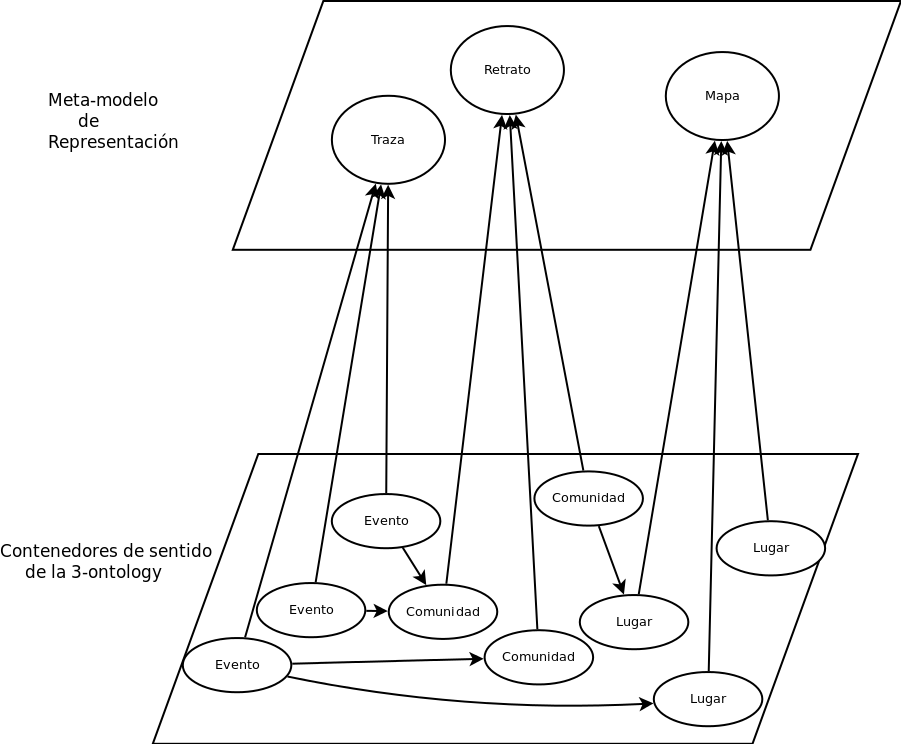
\includegraphics[scale=.5]{images/metamodelo3ontology.png}
	\caption{Meta-modelo de la \textit{3-Ontology}}
	\label{fig:metamodelo3ontology}
\end{figure}

% %Modelo general donde se muestran las contenedores de sentido, representación del darse-cuenta colaborativo, SR, output de un SR.

Los SR utilizan información referente sobre la interacción entre usuarios e ítems. En la Figura \ref{fig:flujodedatos3ontology} se muestra el flujo de datos propuesto para la construcción de un SR de películas basándose en la representación de la \textit{3-Ontology}. Se propone que la entrada de un SR son una traza, un retrato y un mapa. Luego se realiza un conjunto de operaciones pertenecientes a la lógica de la\textit{ 3-Ontology} que permite obtener los eventos, lugares y comunidades de interés para el cálculo de la recomendación. Posteriormente, el SR procesa la información para generar comunidades (recomendación de personas y/o grupos) e ítems (recomendación de ítems). Para el caso particular de recomendación de películas basado en eventos de tipo \textit{rating}  para \textit{Movielens} se tendrían las siguientes pasos:

\begin{enumerate}
	\item Definir la traza como todos de eventos de tipo \textit{rating} y \textit{tagging} del sistema, una comunidad como todos los usuarios que han colocado un \textit{rating} o \textit{tag} a una o varias películas y un mapa como todas las películas que han sido sujeto de interacción del usuario.
	\item Aplicar un conjunto de operaciones de la lógica de la \textit{3-Ontology} para obtener solo los eventos de tipo \textit{rating}, usuarios y películas relevantes para el cálculo de la recomendación para un usuario activo.
	\item El SR utilizando alguna heurística o algoritmo de predicción realiza el cálculo de la preferencia que colocaría el usuario activo. Se seleccionan los ítems con mayor valor de preferencia para ser recomendados.
\end{enumerate}

Es importante señalar que la lógica de la \textit{3-ontology} provee métodos que apoyan a dos de las etapas descritas por \cite{Adomavicius:2011} para los CARS como son las de pre y post-filtrado de eventos permitiendo mejorar el proceso de recomendación mediante el uso de información contextual. Para el pre-filtrado se proveen métodos de obtención de eventos dado algún patrón temporal como días de la semana y fines de semana. Por otro lado, una vez calculada la lista de recomendaciones se puede post-filtrar por algún criterio contextual. Otra forma es pre-filtrar es por tipo de eventos dependiendo de las posibles interacciones que la aplicación provee al usuario (por ejemplo utilizar solo los eventos de tipo \textit{tagging}).

\begin{figure}[tp]
	\centering
	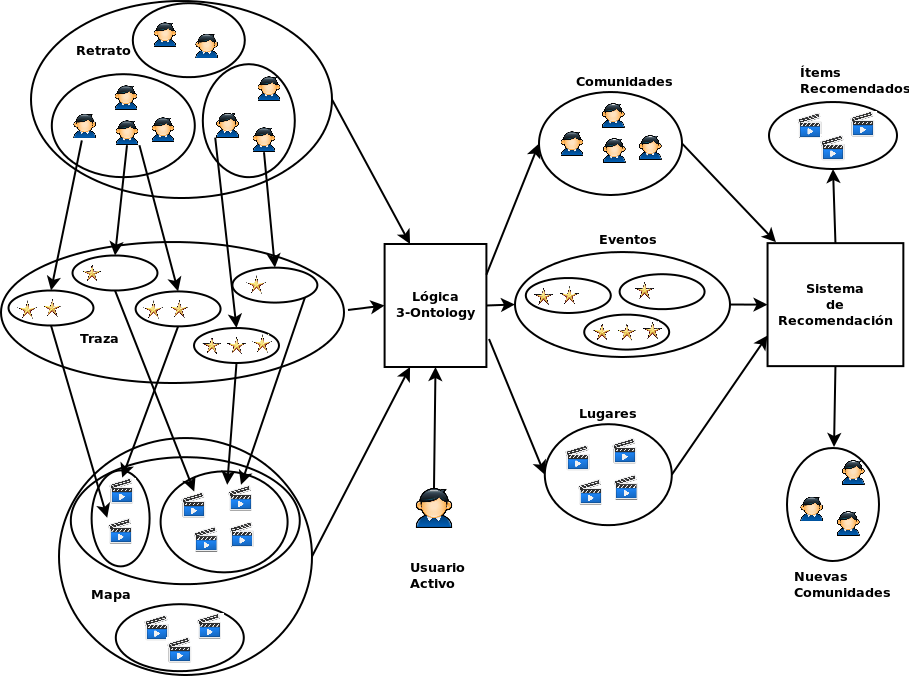
\includegraphics[scale=.5]{images/diagramdeflujopropuesto.png}
	\caption{Flujo de datos propuesto}
	\label{fig:flujodedatos3ontology}
\end{figure}

\subsubsection{Trazas}

Las trazas (ver sección \ref{marco:3ontology}) corresponden a una representación de eventos relacionados temporalmente. Formalmente una traza $T_r$ se define como una estructura con una relación de orden parcial $\prec$ sobre el conjunto potencia de los eventos $E$. 

\begin{equation}
\label{modelo:trazas}
	T_r = (\mathcal{P}(E),\prec)
\end{equation}

Las funciones que se definen sobre las trazas para obtener las relaciones entre los eventos pueden ser temporales, por usuario, tipo de interacción e ítem. Las relaciones temporales entre eventos se definen formalmente como una función $f_t$ con dominio en el tiempo $T$  y recorrido el conjunto potencia de una traza $T_r$. Esto permite obtener subconjuntos de eventos relacionados temporalmente.

\begin{equation}
\label{modelo:operaciontemporal}
	\begin{aligned}
		f_t\colon& T \rightarrow \mathcal{P}(T_r)\\
		& t \rightarrow f_t(t)\\
	\end{aligned}
\end{equation}

Las relaciones de usuarios con eventos se definen formalmente como una función $f_u$ denominada historia de usuario con dominio en el conjunto de usuarios $U$  y recorrido en el conjunto potencia de una traza $T_r$. Esto permite obtener historias de usuario que son definidas por \cite{Ekstrand:2011} como un conjunto de eventos relacionados con un usuario.

\begin{equation}
\label{modelo:operacionusuarios}
	\begin{aligned}
		f_u\colon& U \rightarrow \mathcal{P}(T_r)\\
		& u \rightarrow f_u(u)\\
	\end{aligned}
\end{equation}

Las relaciones de interacciones con eventos se definen formalmente como una función $f_i$ con dominio en el conjunto de posibles interacciones $I$  y recorrido en el conjunto potencia de una traza $T_r$. Esto permite obtener eventos relacionados con un tipo de interacción específico, permitiendo modelar diversas formas de interacción de un usuario con un ítem.

\begin{equation}
\label{modelo:operacioninteraccion}
	\begin{aligned}
		f_i\colon& I \rightarrow \mathcal{P}(T_r)\\
		& i \rightarrow f_i(i)\\
	\end{aligned}
\end{equation}

Las relaciones de ítems con eventos se definen formalmente como una función $f_c$ con dominio en el conjunto de ítems $C$  y recorrido en el conjunto potencia de una traza $T_r$. Esto permite obtener eventos relacionados con un ítem específico.

\begin{equation}
\label{modelo:operacionitem}
	\begin{aligned}
		f_c\colon& C \rightarrow \mathcal{P}(T_r)\\
		& c \rightarrow f_c(c)\\
	\end{aligned}
\end{equation}

\subsubsection{Retratos}

Los retratos (ver sección \ref{marco:3ontology}) corresponden a una representación de las comunidades. Formalmente un retrato $R$ se define como una estructura con una relación de composición $\prec$ sobre el conjunto potencia de comunidades $C$. 

\begin{equation}
\label{modelo:retratos}
	R = (\mathcal{P}(C),\prec)
\end{equation}

La funciones construidas sobre los retratos permiten obtener relaciones entre los usuarios y comunidades. Se define la función $f_u$ con dominio en el conjunto de usuarios $U$ y recorrido en el conjunto potencia de los retratos $R$. Esto permite conocer a que comunidades pertenece un usuario $u$.

\begin{equation}
\label{modelo:funcionusuarioretratos}
\begin{aligned}
		f_u\colon& U \rightarrow \mathcal{P}(R)\\
		& u \rightarrow f_u(u)\\
	\end{aligned}
\end{equation}

\subsubsection{Mapas}

Los mapas (ver sección \ref{marco:3ontology}) corresponden a una representación de los lugares relacionados de forma física y/o virtual. Formalmente un mapa $M$ se define como una estructura con una relación de composición $\prec$ sobre el conjunto potencia de los lugares $L$.  

\begin{equation}
\label{modelo:mapas}
	M = (\mathcal{P}(L),\prec)
\end{equation}

Las funciones que se construyen sobre los mapas permiten obtener relaciones entre los ítems y lugares. Se define la función $f_c$ con dominio en el conjunto de ítems $U$ y recorrido en el conjunto potencia de los retratos $M$. Esto permite conocer a que lugares pertenece un ítem $c$.

\begin{equation}
\label{modelo:funcionitemmapa}
\begin{aligned}
		f_c\colon& C \rightarrow \mathcal{P}(M)\\
		& c \rightarrow f_c(c)\\
	\end{aligned}
\end{equation}



% % Explicación de la representación del darse-cuenta colaborativo de los SR. (Meta nivel referente a las relaciones entre los contenedores básicos).

% % Definición matemática de la representación del darse-cuenta colaborativo.

% % DEfinición de funciones para trace, portrait y maps.


% % Discusión sobre la 3-Ontology apĺicada a SR

\section{Discusi\'on sobre la \textit{3-Ontology} para la representaci\'on de datos en SR}

Para realizar una discusión sobre la representación de datos propuesta se presentan las siguientes criterios y el grado de cumplimiento que provee la representación propuesta.
\begin{itemize}
	\item \textbf{Independencia del dominio}: se refiere a que los SR son independientes del dominio de aplicación. El meta-modelo propuesto de trazas, retratos y mapas permite la abstracción del dominio de aplicación.
	\item \textbf{Perfilamiento de usuarios e ítems}: se refiere a que los SR pueden utilizar información sobre el perfil de los usuarios e ítems.
	\item \textbf{Modelamiento de interacción}: se permite modelar y obtener información sobre distintos tipos interacciones de los usuarios hacia los ítems. La definición propuesta de evento soporta la mayoría de formas de interacción en la Web 2.0.
	\item\textbf{Modelamiento del contexto}: se refiere a la capacidad del SR de obtener información sobre el contexto de la interacción. Esto se logra  situando la interacción en un tiempo, lugar y comunidad.
	\item \textbf{Modelamiento de la comunidad}: se refiere a la capacidad del SR de obtener información sobre la comunidad del usuario como es la reputación y confiabilidad de los usuarios. Dado que los usuarios pertenecen a una comunidad, se pueden determinar medidas de confiabilidad de la recomendación.
	\item \textbf{Modelamiento del espacio}: se refiere a que el SR puede utilizar información referente al espacio tanto físico como virtual. Dado que la representación sitúa al ítem dentro de un lugar, se puede agregar esta información dentro del proceso de recomendación.
\end{itemize}

Dado lo anterior se puede deducir que la capacidad de representación de la \textit{3-ontology} permite modelar la interacción en dominios colaborativos que son el insumo de los SR. En la tabla \ref{tabla:comparacionotrosmodelos} se muestra una comparación con otros modelos presentados en la sección \ref{modelo:trabajorelacionado}. En esta tabla se observa que el modelo de \cite{Babar:2010} permite la independencia del contexto y modelar diversas formas de interacción. De esta forma solo se pueden desarrollar SR de filtrado colaborativo que no utilicen información sobre el usuario e ítem en el proceso de recomendación. Por otro lado, el modelo de \cite{Palomino:2012} a pesar de cumplir con casi todos los criterios de evaluación no tiene una implementación concreta que asegure la eficacia del modelo, solo posee la definición de evento y no construye un meta-modelo de representación sobre los contenedores de sentido que los doten de lógica. Finalmente, cabe destacar que el modelo propuesto demuestra la capacidad de la \textit{3-Ontology} como meta-modelo para representar ambientes colaborativos.

\begin{table}[H]
\caption{Comparación con otros modelos propuestos}
\label{tabla:comparacionotrosmodelos}
\begin{center}
	\begin{tabular}{|>{\centering\arraybackslash}p{3cm}  | >{\centering\arraybackslash}p{2cm}  |>{\centering\arraybackslash}p{2cm} |>{\centering\arraybackslash}p{2cm} |>{\centering\arraybackslash}p{2cm} |}
	\hline	& \multicolumn{4}{c|}{Modelos} \\	
	
	\hline Características	 				 				& Modelo OLAP \cite{Adomavicius:2001}  & Modelo de \cite{Babar:2010} & Modelo de \cite{Palomino:2012} & Modelo Propuesto \\ 
	\hline Independencia del dominio 		 				&   & X & X & X  \\ 
	\hline Perfilamiento de usuarios e ítems 				& X &   &   & X \\ 
	\hline Modelamiento de interacción 						&   &   & X & X \\ 
	\hline Modelamiento del contexto						& X & X & X & X \\ 
	\hline Modelamiento de la comunidad 					&   &   & X & X \\ 
	\hline Modelamiento del espacio					 		&   &   & X & X \\ 
	\hline 
	\end{tabular} 
\end{center}
\end{table}

Por otro lado este modelo resuelve varios de los problemas abordados en este trabajo de tesis:

\begin{enumerate}
	\item \textit{Los cambios en la Web 2.0 y la forma en que los usuarios interactúan con esta. Además, existe dificultad para modelar múltiples interacciones para que estas sean usadas por los SR \citep{Babar:2010}}: el modelo propuesto en este trabajo permite representar cualquier forma de interacción usuario-ítem en una aplicación colaborativa. Esto se logra gracias a la definición de evento propuesta que acepta cualquier valor (real, numérico, nominal, etc) entre la interacción usuario-ítem. 
	\item \textit{Los SR para obtener mejores resultados sobre un dominio específico se acopla demasiado a la data \citep{Babar:2010}. Esto provoca una sobre-especialización del SR, dificultando la posibilidad de reutilizar la solución en otro dominio de aplicación dentro de la empresa}: el modelo presentado permite representar los datos bajo un esquema común que logra un bajo acoplamiento hacia los algoritmos de recomendación subyacentes. Esto permite utilizar distintos algoritmos de recomendación sin la necesidad de realizar una representación distinta de los datos.
	\item \textit{Un SR puede degradar sus resultados en el tiempo debido a cambios en la data referente a la interacción  de los usuarios por lo que debería ser cambiado por otro}: el modelo presentado permite re-entrenar algoritmos mediante la misma representación basada en la \textit{3-ontology} utilizando otros datos asegurando así una mejora continua del rendimiento de los SR.
	\item \textit{Las mejoras obtenidas en los algoritmos son difíciles de generalizar para todos los usuarios del sistema,  por ejemplo algunos usuarios pueden usar un campo muy reducido de opciones de interacción y otros más}: el modelo permite obtener mediante las trazas eventos relevantes a un usuario específico y realizar el cálculo de la recomendación, de esta forma se puede determinar que SR utilizar dado el comportamiento del usuario y el tipo de interacción que más utiliza.
\end{enumerate}

%\section{Resumen}
%
%En este capítulo se realizó la definición formal de la representación de datos propuesta basado en el \textit{framework 3-Ontology}. Se definieron cada uno de los conceptos como son los usuarios, ítems y los contenedores de sentido. Luego se definen formalmente las tres formas de representación que dotan de lógica a la \textit{3-Ontology} trazas, mapas y retratos. Finalmente, se realizó una discusión que demuestra que el modelo propuesto abarca más dimensiones que las representaciones anteriores y resuelve los problemas planteados en este trabajo de tesis.


%
%\begin{lstlisting}[caption = Interface Event]
%/**
%* Interfaz que representa el comportamiento básico de un evento basado en el framework
%* conceptual 3-Ontology
%*
%*/
%public interface Event {
%   /**
%    * Obtiene el identificador del usuario
%    * @return id del usuario
%    */
%   long getUserId();
%   /**
%    * Obtiene el identificador del item
%    * @return id del item
%    */
%   long getItemId();
%   /**
%    * Obtiene una marca temporal del evento
%    * @return timestamp
%    */
%   long getTimestamp();
%   /**
%    * Obtiene la valorización realizada por el usuario al item. Este puede ser de cualquier clase.
%    * @return valor del evento
%    */
%   <T> T getValue();
%}
%\end{lstlisting}












